\documentclass[border=12pt]{standalone}
\usepackage{tikz}
\usetikzlibrary{calc, intersections, through}

\begin{document}
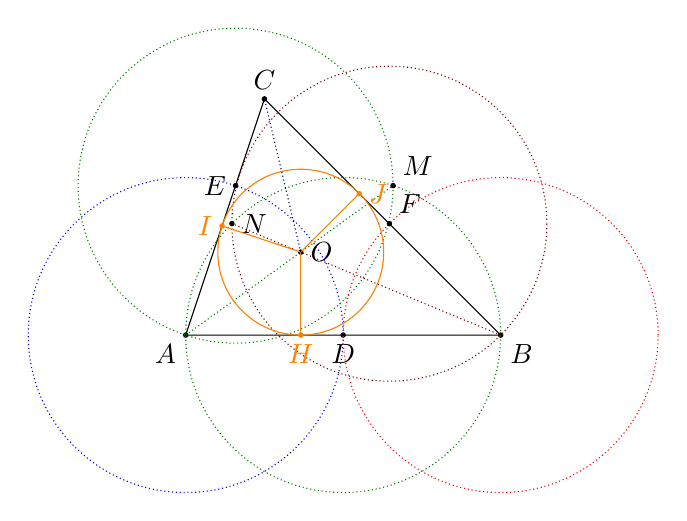
\begin{tikzpicture}[scale=1]

% 定义三角形顶点
\coordinate (A) at (0,0);
\coordinate (B) at (4,0);
\coordinate (C) at (1,3);

% 绘制三角形ABC
\draw[black] (A) -- (B) -- (C) -- cycle;

% 标记点
\fill (A) circle(1pt) node[below left] {$A$};
\fill (B) circle(1pt) node[below right] {$B$};
\fill (C) circle(1pt) node[above] {$C$};

% 构造角A的平分线
% 以A为圆心,半径2cm画弧交AB和AC于D、E
\draw[densely dotted, blue, name path=arcA] (A) circle(2);
\path[name path=AB] (A) -- (B);
\path[name path=AC] (A) -- (C);
\path[name intersections={of=arcA and AB, by={D}}] ;
\fill (D) circle(1pt) node [below] {$D$};
\path [name intersections={of=arcA and AC, by={E}}];
\fill (E) circle(1pt) node [left] {$E$};

% 以D、E为圆心画弧交于M,连接AM为角平分线
\draw[densely dotted, green!50!black, name path=arcD] (D) circle(2); % 圆弧arcD
\draw[densely dotted, green!50!black, name path=arcE] (E) circle(2); % 圆弧arcD
\path[name intersections={of=arcD and arcE, by={M}}];
\draw[densely dotted, green!50!black, name path=AM] (A) -- (M);
\fill (M) circle(1pt) node [above right] {$M$};

% 构造角B的平分线
% 以B为圆心,半径2cm画弧交BC于F
\draw[densely dotted, red, name path=arcB] (B) circle(2);
\path[name path=BC] (B) -- (C);
\path[name intersections={of=arcB and BC, by={F}}];
\fill (F) circle(1pt) node [above right] {$F$};

% 以D、F为圆心画弧交于N,连接BN为角平分线
\draw[densely dotted, red!50!black, name path=arcF] (F) circle(2);
\path[name intersections={of=arcD and arcF, by={N}}];
\draw[densely dotted, red!50!black, name path=BN] (B) -- (N);
\fill (N) circle(1pt) node [right] {$N$};
\path[name intersections={of=AM and BN, by={O}}]; % 确定外心O
\fill (O) circle(1pt) node [right] {$O$};

\coordinate (H) at ($(A)!(O)!(B)$);
\coordinate (I) at ($(A)!(O)!(C)$);
\coordinate (J) at ($(B)!(O)!(C)$);
\fill (H) [orange]circle(1pt) node [below] {$H$};
\fill (I) [orange]circle(1pt) node [left] {$I$};
\fill (J) [orange]circle(1pt) node [right] {$J$};
\draw[orange] (O) -- (H);
\draw[orange] (O) --  (I);
\draw[orange] (O) -- (J);

\node[draw=orange, circle through=(H), inner sep=0] at (O) {}; % 绘制内切圆
\draw[densely dotted, blue!50!black] (O) -- (C);

\end{tikzpicture}
\end{document}